\documentclass[12pt]{article}
\usepackage[a4paper,margin=1in]{geometry}
\usepackage{lmodern}
\usepackage{hyperref}
\usepackage{svg}
\usepackage{graphicx}
\hypersetup{colorlinks=true, urlcolor=blue}

\begin{document}

\title{Project Proposal: ConversaAI -- Interactive English Language Companion}
\author{
    Azmain Inquaid Haque (230218) \\
    Md. Sabbir Khan (230204) \\
    Summa Arifin (230226)
}
\date{\today}
\maketitle

\section*{Introduction}

In today’s global environment, effective English communication is a crucial skill. This project proposes \textbf{ConversaAI}, a Cross-Platform application designed to facilitate English language learning through real-time, natural, and interactive dialogues. By providing immediate feedback, contextual vocabulary suggestions, and rephrasing guidance, ConversaAI aims to create an immersive digital environment for language improvement.

\section*{Project Objectives}

\begin{itemize}
    \item To develop a Cross-Platform application for English language acquisition via conversational practice.
    \item To leverage modern AI and NLP technologies for grammar correction, vocabulary enrichment, and user guidance.
    \item To offer an extensible and maintainable codebase demonstrating best practices in API and library integration.
\end{itemize}

\section*{Target Audience}

Learners of English as a Second Language (ESL) seeking an interactive, feedback-driven desktop application compatible with Linux systems.

\section*{Proposed Solution Overview}

ConversaAI will simulate a conversational English partner. The system will:
\begin{itemize}
    \item Engage users in context-aware dialogues
    \item Provide instant, actionable feedback on grammar and vocabulary
    \item Suggest improved phrasing to promote fluency
    \item Optionally, support speech recognition and text-to-speech for a more immersive experience
\end{itemize}

\section*{Use Case Diagram}

The following diagram illustrates the key use cases of the ConversaAI system and how the user interacts with it:

\begin{figure}[h!]
    \centering
    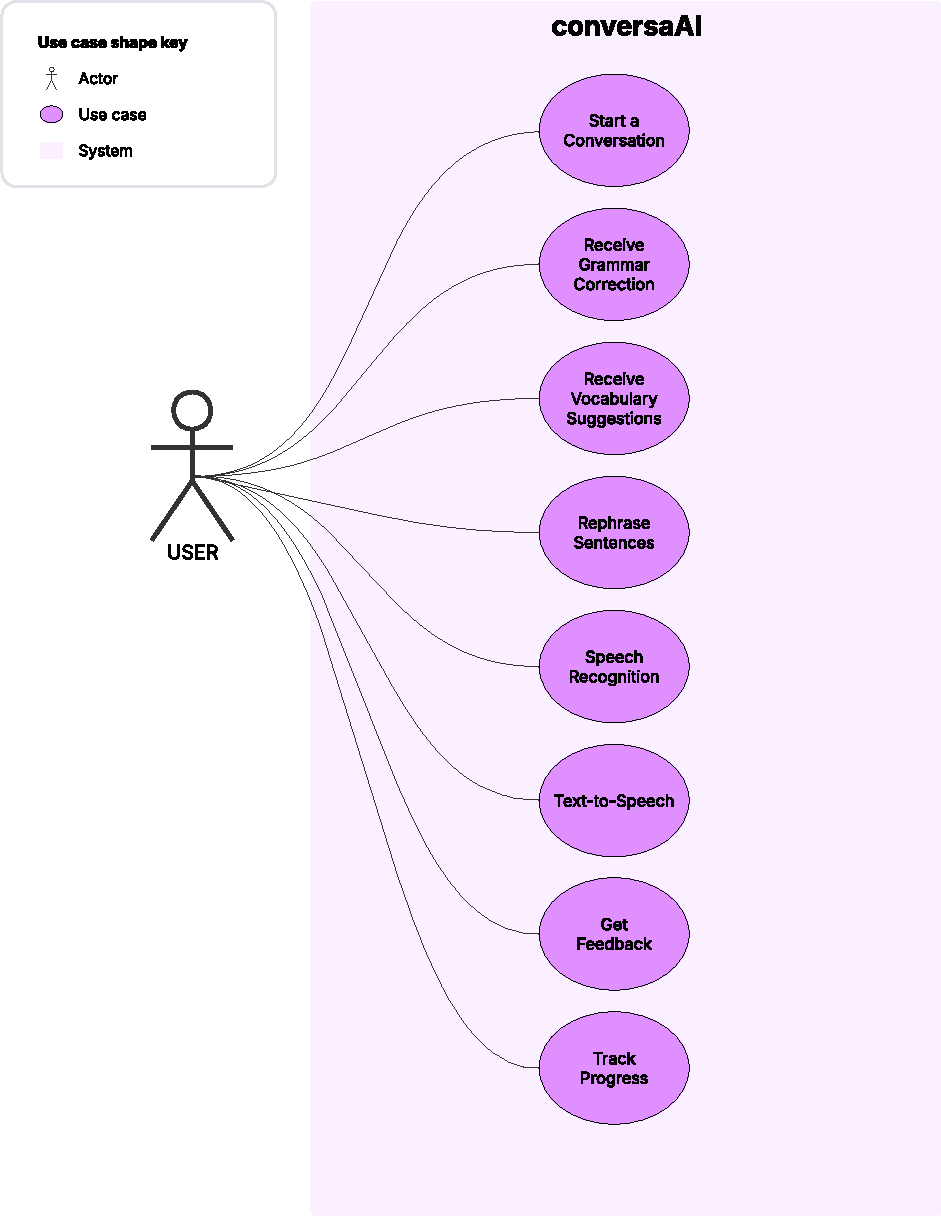
\includegraphics[width=0.8\textwidth]{use_case_diag.pdf}
    \caption{Use Case Diagram for ConversaAI}
    \label{fig:use_case_diagram}
\end{figure}


\section*{Technology Stack and Rationale}

\begin{tabular}{|p{4cm}|p{6cm}|p{4cm}|}
\hline
\textbf{Component} & \textbf{Technology} & \textbf{Rationale / Usage} \\
\hline
Programming Language & Python, Dart & Rapid development, extensive NLP/AI libraries, excellent Linux support \\
\hline
UI Framework & Flutter & Modern, Cross Platform UI, supports complex and responsive interfaces.\\
\hline
Conversational AI and NLP & OpenAI GPT API \newline OR Hugging Face Transformers & For natural dialogue, grammar correction, vocabulary suggestion, contextual feedback via modern NLP models \\
\hline
Speech Recognition & Coqui STT/TTS \newline OR Google Speech APIs & Adds spoken conversation capabilities; open-source options well supported on Linux \\
\hline
Async Processing & Python asyncio \newline or Trio & Efficient real-time message exchange between UI and AI modules \\
\hline
Packaging \& Distribution & PyInstaller \newline or linuxdeployqt & Bundles application and dependencies for easy deployment on Linux systems \\
\hline
\end{tabular}

\section*{Device and System Requirements}

\noindent \textbf{Minimum:}
\begin{itemize}
    \item Linux OS (e.g., Ubuntu 20.04+)
    \item Dual-core 2GHz 64-bit CPU
    \item 4GB RAM
    \item 500MB free disk space
    \item Internet connection for API access
\end{itemize}

\noindent \textbf{Recommended:}
\begin{itemize}
    \item Quad-core 2.5GHz 64-bit CPU or higher
    \item 8GB+ RAM
    \item 2GB+ disk space
    \item Full HD display
    \item Broadband internet (25Mbps+), microphone/speakers for voice features
\end{itemize}

\section*{Expected Outcomes}

\begin{itemize}
    \item Functional Cross-Platform application for English conversation practice with real-time, AI-driven feedback.
    \item Demonstration of API and library integrations -- especially with state-of-the-art NLP tools.
    \item Extensible foundation for further feature development (e.g., additional languages, richer speech interaction).
\end{itemize}

\section*{Conclusion}

This proposal details the development plan for ConversaAI, focusing on a robust, modern tech stack optimized for Linux. The application will present an effective solution for English language learners, utilizing current advances in natural language processing and desktop software design.
\end{document}
